\documentclass[a4paper,11pt]{article}
\usepackage[utf8]{inputenc}
\usepackage[russian]{babel}
\usepackage[T1]{fontenc}
\usepackage{amssymb,amsmath,graphicx,indentfirst}

\author{Иван Веселов}
\title{Курс kiev-clrs -- Лекция 14. Конкурентный анализ}
\date{2009 г.}

\begin{document}

\maketitle
\tableofcontents
\newpage

\setlength{\parskip}{1ex plus 0.5ex minus 0.2ex}

\section{План лекции}
\begin{itemize}
\item Самоорганизующиеся списки
\item Эвристика MTF (move to front)
\item Конкурентный анализ MTF
\end{itemize}

\section{Самоорганизующиеся списки}

Рассмотрим список $L$ из $n$ элементов.
\begin{itemize}
\item Операция $Access(x)$ стоит $rank_L(x)$, то есть расстояние
  от головы списка до элемента $x$
\item Соседние элементы списка можно менять местами за стоимость 1.
\end{itemize}

\begin{figure}[ht]
  \centering
  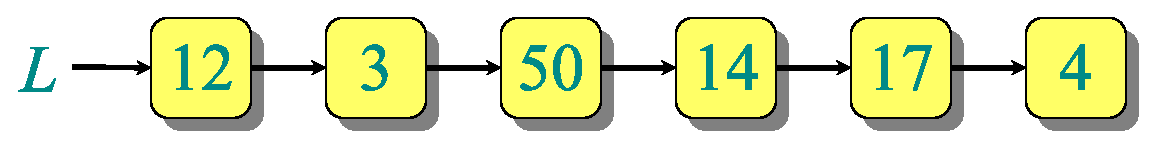
\includegraphics[width=3in]{lecture14/list.eps}
  \caption{Список L}
  \label{fig:list}
\end{figure}

Пример:
\begin{itemize}
\item доступ к элементу с ключом 14 (четвёртый элемент) стоит 4
\item обмен элементов с ключами 3 и 50 стоит 1
\end{itemize}

Поскольку стоимость доступа зависит от позиции элемента, то для уменьшения общих
расходов следует передвинуть те элементы, доступ к которым требуется наиболее
часто, в начало списка.

\section{Онлайн и оффлайн алгоритмы}

\textbf{Определение}: последовательность операций $S$ предоставляется по одной
операции за раз. Для каждой из операций \emph{онлайн-алгоритм} $A$ должен
выполнять эту операцию незамедлительно, безо всякого знания о последующих
операциях последовательности. Пример: игра тетрис.

\emph{Оффлайн-алгоритм} может использовать знание сразу о всей
последовательности операций (``видит'' всю последовательность $S$ наперёд).

Наша цель -- минимизировать полную стоимость всех операций алгоритма $C_A(S)$

\section{Анализ наихудшего и среднего случаев}

Проведём анализ наихудшего случая:

В худшем случае у нас есть противник, который знает как расположены элементы в
списке и с целью максимизации времени будет намеренно запрашивать каждый раз тот
элемент, который расположен в списке последним. Таким образом, оценка полной
стоимости такова:
$$
C_A(S) = \Omega(|S| \cdot n)
$$

Теперь проведём анализ среднего случая.

Предположим что к элементу $x$ доступаются с вероятностью $p(x)$, тогда
ожидаемая общая стоимость будет равна:

$$
E(C_A(S)) = \sum_{x \in L} p(x) \cdot rank_L(X)
$$

это минимизируется, если элементы отсортированы в порядке уменьшение
вероятности.

Эвристики:
\begin{itemize}
\item поддерживать массив, в котором будет хранится количество доступов для
  каждого элемента и поддерживать этот массив в отсортированном состоянии вместе
  с исходным списком элементов
  
\item перемещение в начало (\emph{move to front}, \emph{MTF}) -- после доступа к
  элементу передвинуть его в самое начало списка. Это удвоит стоимость доступа,
  т.к. после доступа нужно будет совершить $rank_L(X)$ перестановок:
  
  $$
  cost = 2 \cdot rank_L(X)
  $$

  Эта стратегия обладает так называемым \emph{свойством локальности}, то есть
  хорошо проявляет себя для последовательностей, конкретные элементы которых
  запрашиваются несколько раз подряд или же просто рядом по времени. Как
  показывает опыт, такие последовательности весьма часто встречаются на
  практике.

\end{itemize}

\section{Конкурентный анализ}

Онлайн-алгоритм $A$ называется $\alpha$-конкурентным, если существует такая
константа $k$, что для всех последовательностей операций $S$ выполняется
неравенство:

$$
C_A(S) \leqslant \alpha \cdot C_{OPT}(S) + k
$$

где OPT -- оптимальный оффлайн алгоритм (``алгоритм Бога'').

Замечательным результатом Тарджана и Слейтора является следующая теорема.

\textbf{Теорема:} Стратегия MTF является 4-конкурентным для самоорганизирующихся
списков.

\textbf{Доказательство:} Введём некоторые обозначения. Пусть

$L_i$ -- это список $L$ после $i$-й операции доступа по алгоритму MTF

$L_i^*$ -- это список $L$ после $i$-й операции доступа по алгоритму OPT

$c_i$ -- стоимость $i$-й операции по алгоритму MTF $=2 \cdot rank_{L_{i-1}}(x) $

$c_i^*$ -- стоимость $i$-й операции по алгоритму OPT $= rank_{L_{i-1}}(x) + t_i$

где $t_i$. количество перестановок, которое выполняет алгооритм OPT.

Теперь нам нужно каким-то образом сравнивать два списка: MTF и OPT, то есть два
списка, которые получаются на $i$-х шагах алгоритмов MTF и OPT соответственно.

Идея состоит в использовании потенциальной функции, которая будет измерять
разницу между списками с помощью количества \emph{инверсий}.

Определим потенциальную функцию $\Phi \colon \lbrace L_i \rbrace \to \mathbb{R}$
следующим образом:

\begin{align*}
\Phi(L_i) &= 2 \cdot
   | \{ (x, y) \colon x \prec_{L_i} y \text{ и } y \prec_{L_i^*} x \} | \\
          &= 2 \cdot \# \text{инверсий}
\end{align*}

\begin{figure}[ht]
  \centering
  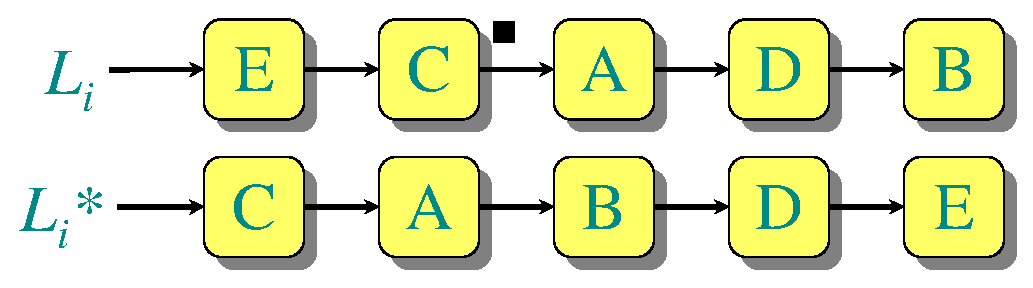
\includegraphics[width=3in]{lecture14/inversions.eps}
  \caption{Подсчёт количества инверсий}
  \label{fig:inversions}
\end{figure}

Пример:
$$
\Phi(L_i) = 2 \cdot \{ (E,C), (E,A), (E,D), (E,B), (D,B)\} = 10
$$

Проверим свойства, которые должны присутствовать у потенциальной функции по
определению:

\begin{itemize}
\item $\Phi_i \geqslant 0 \forall i$, поскольку это рамзер множества и он не
  может быть отрицательным
\item $\Phi_0 = 0$ в случае если оба алгоритма (MFT и OPT) начинают работать с
  одним и тем же списком
\end{itemize}

Насколько может измениться потенциал после одной перестановки соседних
элементов? Он может либо увеличится на единицу, либо уменьшится на единицу.
Поскольку перестановка соседних элементов ничего не меняет во взаимном
расположении всех остальных элементов, то изменения будут касаться только этих
двух элементов. А именно: перестановка может либо сделать их следующим в
одинаковом порядке (уменьшит количество инверсий), либо наоборот -- увеличит
количество инверсий на единицу. Таким образом, $\Delta\Phi = \pm 2$

Что происходит при доступе к элементу $x$? Чтобы разобраться в этом вопросе
предположим, что $i$-я операция доступается к элементу $x$ и введём следующие
множества:
\begin{gather*}
A = \{ y \in L_{i-1} : y \prec_{L_{i-1}} x \text{ и } y \prec_{L_{i-1}^*} x \}
\\
B = \{ y \in L_{i-1} : y \prec_{L_{i-1}} x \text{ и } y \succ_{L_{i-1}^*} x \}
\\
C = \{ y \in L_{i-1} : y \succ_{L_{i-1}} x \text{ и } y \prec_{L_{i-1}^*} x \}
\\
D = \{ y \in L_{i-1} : y \succ_{L_{i-1}} x \text{ и } y \succ_{L_{i-1}^*} x \}
\end{gather*}

\begin{figure}[ht]
  \centering
  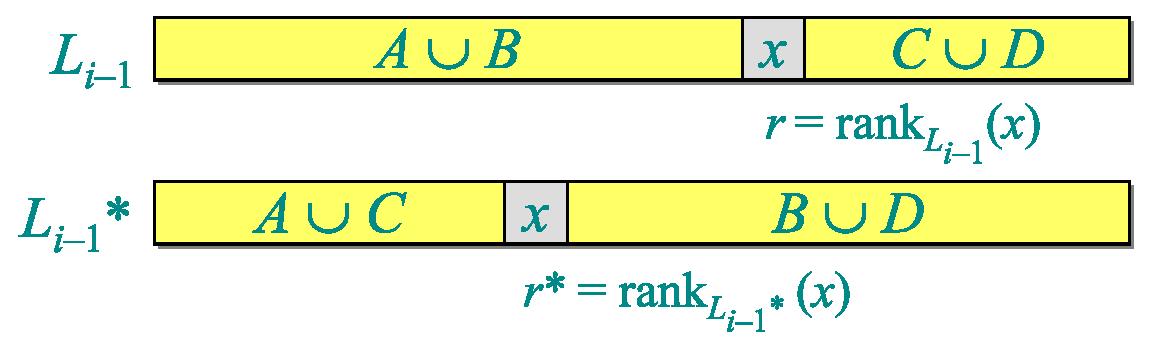
\includegraphics[width=3in]{lecture14/sets.eps}
  \caption{Множества A, B, C, D}
  \label{fig:sets}
\end{figure}

Объяснение: слева от элемента $x$ в $L_{i-1}$ лежат элементы из $A$ и из $B$,
т.к. нам не важно, где именно они находятся в $L_{i-1}^*$, главное, что и для
$A$ и для $B$ выполняется $y \prec_{L_{i-1}} x$, что позволяет нам заключить,
что их элементы находятся слева от элемента $x$ в $L_{i-1}$. Аналогичные
рассуждения могут быть проведены и для остальных трёх частей.

Введём $r$ и $r^*$ -- ранги $x$ в двух списках. Несложно заметить, что:
\begin{gather*}
  r = |A| + |B| + 1 \\
  r^* = |A| + |C| + 1
\end{gather*}

Когда MFT передвигает элемент в начало списка он создаёт $|A|$ инверсий и
удаляет $|B|$ инверсий. Каждая же перестановка соседних элементов в процессе
работы OPT создаёт как максимум одну инверсию (как мы показали ранее).

Таким образом разница потенциалов (увеличение числа инверсий) ограничена сверху:
$$
\Phi(L_i) - \Phi(L_{i-1}) \leqslant 2 \cdot (|A| - |B| + t_i)
$$


Определим амортизационную стоимость $\hat{c}_i$ $i$-й операции по отношению к
функции $\Phi$ равна:
\begin{align*}
\hat{c}_i &= c_i + \Phi(L_i) - \Phi(L_{i-1})  \\
  &\leqslant 2r + 2(|A| - |B| + t_i) \\
  &= 2r + 2(|A| - (r - 1 - |A|) + t_i) \\
  &= 2r + 4|A| - 2r + 2 + 2t_i \\
  &= 4|A| + 2 + 2t_i \\
  &\leqslant 4(r^* + t_i) \text{, поскольку } r^* = |A| + |C| + 1 \geqslant |A| +
  1 \\
  &= 4c_i^*
\end{align*}

Подсчитаем суммарную стоимость операций при алгоритме MTF:
\begin{align*}
  C_{MTF}(S) &= \sum_{i=1}^{|S|} c_i \\
  &= \sum_{i=1}^{|S|} \hat{c}_i + \Phi(L_{i-1}) - \Phi(L_i) \\
  &\leqslant (\sum_{i=1}^{|S|} 4c_i^*) + \Phi(L_0) - \Phi(L_{|S|}) \\
  &\leqslant 4 \cdot C_{OPT}(S) \text{, поскольку } \Phi(L_0) = 0, \Phi(L_{|S|}
  \geqslant 0)
\end{align*}

что и требовалось доказать.

\textbf{Дополнение}: если считать, что перемещения в начала списка  ``бесплатными'', предполагая,
что мы можем сделать их быстро, прямо меняя местами заданный элемент с началом
списка, то тогда MTF является 2-конкурентным алгоритмом, то есть всего в два
раза хуже оптимального оффлайн алгоритма.

Рассмотрим случай, когда $L_0 \neq L_0^*$. Тогда в наихудшем случае $\Phi_0 =
\Theta(n^2)$ и, таким образом, $C_{MTF}(S) \leqslant 4\cdot C_{OPT}(S) +
\Theta(n^2)$, но это всё ещё 4-конкурентность, т.к. $n^2$ -- константа, если
$|S| \rightarrow \infty$, а по определению конкурентности допускается
константа-слагаемое в правой части.

\end{document}


